\section{Consuntivazione}

\subsection{Milestones:}
\begin{itemize}
    \item Release versione 0.0.4 (Completa al: 75\%)
\end{itemize}

\subsection{Attività svolte}

\begin{table}[ht]
    \begin{tabularx}{\textwidth}{X l l}
        
        \rowcolor{gray!30} \textbf{Attività} & \textbf{Stato} & \textbf{Ruolo}\\
        
        \hline
        standardizzato repository delle \textbf{NdP} & completato & Amministratore\\
        inizializzato repository del \textbf{PoC} & completato & Amministratore\\
        \end{tabularx}
    \caption{Lista delle attività svolte durante lo sprint}
\end{table}


\begin{table}[ht]
    \begin{tabularx}{\linewidth}{X|rrrrrrr}
    \rowcolor{gray!30}& Re & Amm & An & Pro & Prog & Ver & tot \\
    \hline
    Bonavigo Michele                        & 3,5 & 0 & 0 & 0 & 0 & 0,3  & 3,8 \\
    \rowcolor{gray!10}Casarotto Mattia      & 0 & 0 & 0 & 0 & 0 & 0  & 0 \\
    Massarenti Alessandro                   & 0 & 0,8 & 0 & 0 & 0 & 0,55  & 1,35 \\
    \rowcolor{gray!10}Peron Samuel          & 0 & 0 & 0 & 0 & 0 & 0 & 0 \\
    Pierobon Luca                           & 0 & 0,3 & 0 & 0 & 0 & 0 & 0,3 \\
    \rowcolor{gray!10}Romano Davide         & 0 & 0 & 0 & 0 & 0 & 0 & 0 \\
    Zarantonello Giorgio                    & 0 & 0 & 0 & 0 & 0 & 0 & 0 \\
    \hline                                  & 3,5 & 1,1 & 0 & 0 & 0 & 0,85 & 
    \end{tabularx}
    \caption{\label{ruoli-persone}Spartizione dei ruoli e ore svolte durante lo sprint}
\end{table}

\begin{center}
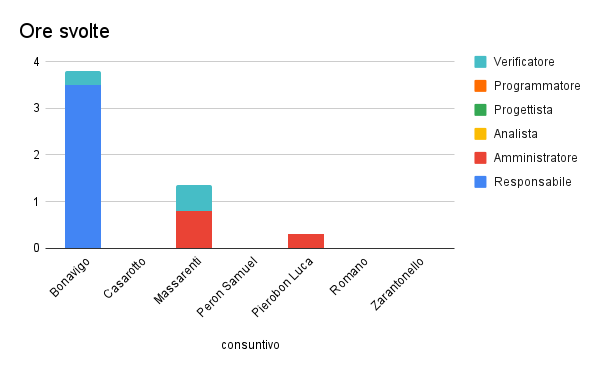
\includegraphics[width=12cm]{img/ore-svolte.png}
\end{center}

\begin{table}[ht]
    \begin{tabularx}{\linewidth}{X|l|l}
    \rowcolor{gray!30}& Ore & Costo \\
    \hline
    
    Responsabile & 3,5 & € 105,00 \\
    \rowcolor{gray!10}Amministratore & 1,1 & € 22,00 \\
    Analista & 0 & € 0,00 \\
    \rowcolor{gray!10}Progettista & 0 & € 0,00 \\
    Programmatore & 0 & € 0,00 \\
    \rowcolor{gray!10}Verificatore & 0,85 &€ 12,75 \\
    totale & 5,45 & € 139,75 \\
    \end{tabularx}
    \caption{\label{costi-ruolo}Spartizione dei ruoli e ore svolte durante lo sprint}
\end{table}


Avendo quindi consumato €139,75\footnote{Si veda tabella \ref{costi-ruolo}} del budget durante questo sprint, rimangono ancora a disposizione € 12640,75 per gli sprint seguenti.

\subsection{Trend e riflessioni}

\begin{figure}[ht]
    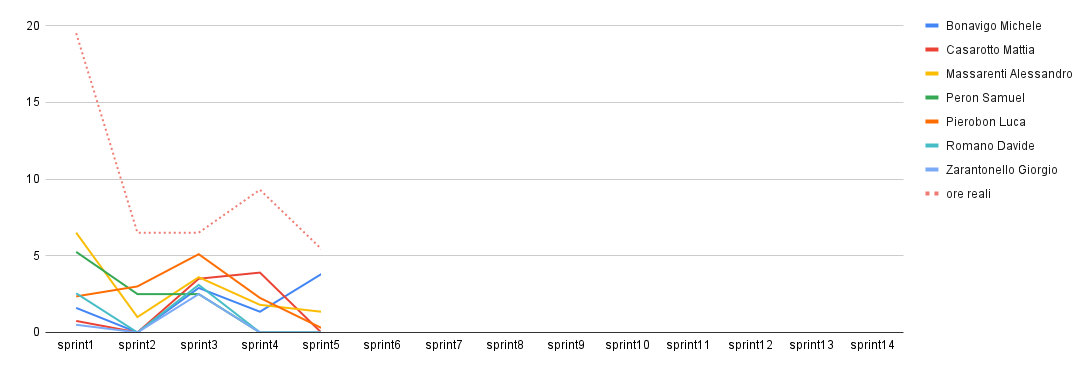
\includegraphics[width=\linewidth]{img/andamento.png}
    \caption{Andamento ore utilizzate nei vari sprint}\label{img:andamento}
\end{figure}

Si può notare nella figura \ref{img:andamento} un trend negativo, va però contestualizzato con l'inizio del periodo natalizio.

Probabilmente nello sprint 6 vedremo l'inizio di un trend in ascesa.

\subsection{Difficoltà e problemi di sprint}

Alcune questioni sono risultate durante questo sprint:

\begin{itemize}
    \item nello sviluppo del \textbf{PoC} abbiamo incontrato difficoltà a comprendere completamente il funzionamento del sistema \textit{CORS} del browser;
    \item il proponente ha cambiato il supporto hardware per problemi di reperimento dello stesso, questo apporterà modifiche all'analisi dei requisiti;
    \item difficoltà nella gestione delle attività durante le vacanze.
\end{itemize}

Queste verranno discusse in sede di preparazione del prossimo sprint.
